\documentclass[11pt]{article}
\usepackage[margin=1in]{geometry}
\usepackage{mathpazo}
\usepackage{amsmath,amssymb}
\usepackage{microtype}
\usepackage{booktabs}
\usepackage{graphicx}
\usepackage[dvipsnames]{xcolor}
\usepackage{tikz}
\usetikzlibrary{positioning,arrows.meta,calc,fit,backgrounds}
\usepackage[most]{tcolorbox}
\usepackage{enumitem}
\usepackage{listings}
\usepackage[font=small,labelfont=bf]{caption}
\usepackage{hyperref}
\hypersetup{colorlinks=true,linkcolor=MidnightBlue,citecolor=MidnightBlue,urlcolor=MidnightBlue}
\usepackage{cleveref}
\urlstyle{tt}
\def\UrlBreaks{\do\_\do/\do.}
\newcommand{\file}[1]{\nolinkurl{#1}}
\newcommand{\code}[1]{\texttt{#1}}
\newcommand{\mhh}{m_{hh}}
\newcommand{\bw}{\boldsymbol{\omega}}
\newcommand{\bp}{\boldsymbol{p}}
\newcommand{\bx}{\boldsymbol{x}}
\newcommand{\data}{\mathcal{D}}

\definecolor{trainable}{HTML}{1B6CA8}
\definecolor{physics}{HTML}{2E933C}
\definecolor{datac}{HTML}{7B4EA3}
\definecolor{warn}{HTML}{C0392B}

\newtcolorbox{keyidea}[1][]{enhanced,breakable,colback=physics!6,colframe=physics!70!black,
  fonttitle=\bfseries,title={#1},boxrule=0.6pt,arc=2pt,left=6pt,right=6pt}
\newtcolorbox{aside}[1][]{enhanced,breakable,colback=trainable!5,colframe=trainable!70!black,
  fonttitle=\bfseries,title={#1},boxrule=0.6pt,arc=2pt,left=6pt,right=6pt}
\newtcolorbox{assume}[1][]{enhanced,breakable,colback=datac!5,colframe=datac!70!black,
  fonttitle=\bfseries,title={#1},boxrule=0.6pt,arc=2pt,left=6pt,right=6pt}
\newtcolorbox{watch}[1][]{enhanced,breakable,colback=warn!5,colframe=warn!70!black,
  fonttitle=\bfseries,title={#1},boxrule=0.6pt,arc=2pt,left=6pt,right=6pt}
\setlist{itemsep=2pt,topsep=3pt}
\setlength{\emergencystretch}{3em}

\lstset{language=Python, basicstyle=\ttfamily\small, columns=fullflexible,
  keepspaces=true, commentstyle=\color{physics!70!black}\itshape,
  keywordstyle=\color{trainable!90!black}\bfseries, stringstyle=\color{datac},
  showstringspaces=false, frame=single, rulecolor=\color{gray!40},
  backgroundcolor=\color{gray!3}, xleftmargin=4pt, xrightmargin=4pt,
  aboveskip=6pt, belowskip=6pt}

\newcommand{\what}{\hat{\boldsymbol{\omega}}}
\newcommand{\bj}{\boldsymbol{j}}
\newcommand{\bC}{\boldsymbol{C}}

\title{\textbf{A Bayesian uncertainty for \texttt{HEFTNet}}\\[4pt]
\large The mixture of linearised Laplace approximations, explained\\[4pt]
\normalsize With the code in \file{dihiggs/laplace.py}, \file{dihiggs/counts.py} and
\file{code/heft_laplace.ipynb}}
\date{October 31, 2026}

\begin{document}
\maketitle

\begin{abstract}
\noindent
This note explains, step by step and for readers who have not met the method before, how
we approximate the posterior density of the parameters of \texttt{HEFTNet} by a mixture of
Gaussians, one about each network of the fine-tuned ensemble, and how that gives a
Bayesian uncertainty for the predicted cross section. It covers the noise model (the
POWHEG spectra are scaled Poisson counts), the linearisation of a network and the
Gaussian posterior it implies, MacKay's evidence approximation for the prior, a property
of \texttt{HEFTNet} that makes the calculation exact and fast, the mixture, the model error,
and the checks. The last section gives the first results. The plan that this implements is
\file{docs/bnn/bnn_plan2.pdf}.
\end{abstract}

\tableofcontents

% ===========================================================================
\section{Why we are doing this}

Bayes' theorem gives the density of the network parameters $\bw$ given the training data
$\data$,
\begin{equation}
  p(\bw \mid \data) \propto p(\data \mid \bw)\, \pi(\bw) ,
\end{equation}
and the uncertainty of a prediction follows by propagating that density through the
network. Our Markov chains (Hamiltonian Monte Carlo, following Neal) gave widths of only
0.5\% of the POWHEG noise. \file{bnn_plan2.pdf} shows why: a single chain of $10^3$
iterations could not explore a 3,944-dimensional density whose curvatures differ by a
factor $10^6$ or more, and it stayed near one of the many equally good solutions. The
approach here avoids sampling altogether. It replaces the exact posterior by an
approximation that can be computed with linear algebra, and it builds in the several
solutions by using the 20 networks of the ensemble.

% ===========================================================================
\section{The data are scaled event counts}
\label{sec:counts}

Each POWHEG spectrum is a histogram of 40,000 generated events (about 16,000 for two short
runs), all with the same weight
$q_s$ (in pb) for spectrum $s$. The cross section in bin $k$ is
\begin{equation}
  t_k = q_s\, n_k , \qquad n_k \in \{0, 1, 2, \ldots\} .
\end{equation}
\file{dihiggs/counts.py} recovers $q_s$ and the integers $n_k$ of every spectrum exactly
(\file{docs/counts/counts_note.pdf}). The count $n_k$ is Poisson distributed, so
\begin{equation}
  \mathrm{Var}(t_k) = q_s^2\, \mathrm{Var}(n_k) = q_s^2\, \langle n_k\rangle \approx q_s\, t_k .
\end{equation}
We use $\sigma_k^2 = q_s(t_k + q_s)$: the added $q_s^2$ is the variance of one event, and it
keeps the variance of empty or nearly empty bins from vanishing. The bins of different
spectra, and (up to a negligible multinomial correlation) the bins of one spectrum, are
independent. The 1,814 empty bins, which had been dropped from the training file, are
restored: an empty bin tells us the cross section there is small.

\begin{aside}[Why not $q_s f_k$, the Poisson variance at the prediction?]
For a Poisson likelihood the textbook weight of a bin is $1/(q_s f_k)$, with $f_k$ the
prediction. We tried it. It gives a huge weight to the few bins where a network predicts
a negative or tiny value against a large count: in the first network, two of 274,152 rows
contributed a quarter of the $\chi^2$. Those bins would dominate the curvature in their
directions. The networks were fine-tuned with $q_s(t_k + q_s)$, so we use it here too
(switch \code{VARIANCE\_FROM}).
\end{aside}

% ===========================================================================
\section{The Laplace approximation}

\subsection{The idea}

Near its maximum, almost any smooth, single-peaked density looks like a Gaussian: expand
$\ln p$ to second order about the peak and exponentiate. This is the Laplace approximation.
For a network, the expansion is done most usefully not in $\ln p$ directly but in the
network itself.

\subsection{Linearising the network}

Let $\what$ be a trained network and $\bj(\bx) = \partial f(\bx;\bw)/\partial\bw$ at
$\what$, a vector with one entry per parameter (3,944 for \texttt{HEFTNet}). For $\bw$ near
$\what$,
\begin{equation}
  f(\bx;\bw) \approx f(\bx;\what) + \bj(\bx)^{\mathsf T}(\bw - \what) .
  \label{eq:lin}
\end{equation}
The right-hand side is \emph{linear in the parameters}: it is a linear regression whose
``basis functions'' are the components of $\bj(\bx)$. Everything that follows is the
textbook solution of a linear regression with Gaussian noise and a Gaussian prior.

\begin{keyidea}[A linear regression refresher]
Fit $y_k = \boldsymbol{\phi}_k^{\mathsf T}\boldsymbol{\beta} + \text{noise}$, noise variance
$\sigma_k^2$, with a Gaussian prior of precision matrix $T$ on $\boldsymbol{\beta}$. The
log posterior is
$-\tfrac12\sum_k (y_k - \boldsymbol{\phi}_k^{\mathsf T}\boldsymbol{\beta})^2/\sigma_k^2
- \tfrac12 \boldsymbol{\beta}^{\mathsf T} T \boldsymbol{\beta}$, a quadratic in
$\boldsymbol{\beta}$. The posterior is therefore exactly Gaussian, with precision (inverse
covariance)
\[
  H = \sum_k \frac{\boldsymbol{\phi}_k \boldsymbol{\phi}_k^{\mathsf T}}{\sigma_k^2} + T .
\]
The prediction $\boldsymbol{\phi}^{\mathsf T}\boldsymbol{\beta}$ at a new point is Gaussian
with variance $\boldsymbol{\phi}^{\mathsf T} H^{-1} \boldsymbol{\phi}$. Each data point
adds a ``rank-one'' piece $\boldsymbol{\phi}_k\boldsymbol{\phi}_k^{\mathsf T}/\sigma_k^2$:
more data, or less noisy data, make $H$ larger and the posterior narrower.
\end{keyidea}

\subsection{The posterior and the prediction}

With $\boldsymbol{\phi}_k = \bj_k \equiv \bj(\bx_k)$, a likelihood
$\prod_k \mathcal{N}(t_k; f_k, \sigma_k^2)$ and Neal's prior, which gives each parameter
$i$ in group $g(i)$ (one group per weight matrix or bias vector, 16 for \texttt{HEFTNet}) a
Gaussian of precision $\tau_{g(i)}$, the posterior of the linearised network is Gaussian
about $\what$ with precision
\begin{equation}
  H = G + T, \qquad
  G = \sum_{k=1}^{N} \frac{\bj_k \bj_k^{\mathsf T}}{\sigma_k^2}, \qquad
  T = \mathrm{diag}(\tau_{g(i)}) .
  \label{eq:H}
\end{equation}
$G$ is called the (generalised) Gauss--Newton matrix. It is the curvature of $\chi^2/2$,
except that a term proportional to the residuals $f_k - t_k$ is left out; that term is
small near a good fit, and leaving it out guarantees that $G$ has no negative eigenvalues.
The prediction at $\bx$ is Gaussian with
\begin{equation}
  \text{mean } \mu(\bx) = f(\bx;\what), \qquad
  \text{variance } v(\bx) = \bj(\bx)^{\mathsf T} H^{-1} \bj(\bx) .
  \label{eq:pred}
\end{equation}
This is MacKay's original treatment of Bayesian networks (1992), now called the
``linearised Laplace approximation'' or the ``GLM predictive''. Note that the network is
linearised in the \emph{prediction} as well as in the posterior; that consistency is what
makes the method work well.

\begin{aside}[How the code computes $v$ without inverting $H$]
$H$ is symmetric and positive definite, so it has a Cholesky factorisation $H = LL^{\mathsf T}$
with $L$ lower triangular. Then $v = \bj^{\mathsf T}(LL^{\mathsf T})^{-1}\bj = |L^{-1}\bj|^2$,
and $L^{-1}\bj$ is one triangular solve. For 3,944 parameters the factorisation takes
about a second. Everything is done in double precision, because the eigenvalues of $H$ span
about 13 orders of magnitude.
\end{aside}

% ===========================================================================
\section{The prior: MacKay's evidence approximation}
\label{sec:prior}

The precisions $\tau_g$ control how far the parameters of group $g$ may stray from zero. In
the Markov chains they were sampled. Here we choose them by maximising the
\emph{evidence}, the probability of the data given $\tau$ with the parameters integrated
out, which the Laplace approximation makes available in closed form. Setting its
derivative with respect to $\tau_g$ to zero gives MacKay's fixed-point equations:
\begin{equation}
  \tau_g = \frac{\gamma_g}{\sum_{i\in g}\hat\omega_i^2}, \qquad
  \gamma_g = n_g - \tau_g \sum_{i\in g} \big(H^{-1}\big)_{ii} ,
  \label{eq:mackay}
\end{equation}
with $n_g$ the number of parameters in group $g$.

\begin{keyidea}[What $\gamma$ means]
Along an eigenvector of $G$ with eigenvalue $\lambda$, the data contribute curvature
$\lambda$ and the prior $\tau$. If $\lambda \gg \tau$ the data determine that combination
of parameters; if $\lambda \ll \tau$ the prior does. $\gamma = \sum \lambda/(\lambda +
\tau) = \mathrm{tr}(GH^{-1})$ counts the combinations the data determine: MacKay's ``number
of well-determined parameters''. $\gamma_g$ is its share in group $g$. The first equation
of \cref{eq:mackay} then says: the prior variance $1/\tau_g$ should equal the mean square
of the \emph{well-determined} parameters of the group.
\end{keyidea}

The equations are solved by iteration. Only the diagonal of $H$ changes with $\tau$, so
each iteration is one Cholesky factorisation. The plain iteration overshoots and
oscillates, so each step moves half-way, in $\ln\tau$ (\code{damping = 0.5}). The
expansion point $\what$ is held fixed; strictly it would move a little as $\tau$ changes,
but the prior term is tiny beside the $\chi^2$.

% ===========================================================================
\section{The structure of HEFTNet, and why it makes everything exact and fast}
\label{sec:structure}

\texttt{HEFTNet} is not a generic network. Its output is
\begin{equation}
  f(\bx;\bw) = \sum_{i=1}^{23} C_i(\theta)\, a_i(m_{hh};\bw) ,
  \label{eq:heftnet}
\end{equation}
where the $C_i$ are the known polynomials in the five HEFT parameters $\theta$ and the 23
functions $a_i$ are the outputs of the network, \emph{which sees only} $m_{hh}$. Hence
\begin{equation}
  \bj(\bx) = \sum_i C_i(\theta)\, \frac{\partial a_i(m_{hh})}{\partial\bw}
           = A(m_{hh})^{\mathsf T}\, \bC(\theta),
\end{equation}
with $A(m_{hh})$ the $23\times3{,}944$ Jacobian of the 23 functions. There are only 80
distinct values of $m_{hh}$ (the bins). Writing $A_b$ for bin $b$,
\begin{equation}
  G = \sum_b A_b^{\mathsf T} S_b A_b , \qquad
  S_b = \sum_{k \in \text{bin } b} \frac{\bC_k \bC_k^{\mathsf T}}{\sigma_k^2} ,
  \label{eq:Gfact}
\end{equation}
where $S_b$ is a $23\times23$ matrix that sums over all the training rows in bin $b$. So
$G$ needs 80 Jacobians, not 274,152, and the result is identical (the code checks this
against the row-by-row calculation: they agree to $10^{-15}$). Likewise the prediction
variance is
\begin{equation}
  v(\bx) = \bC(\theta)^{\mathsf T} K_b\, \bC(\theta), \qquad
  K_b = A_b H^{-1} A_b^{\mathsf T} ,
  \label{eq:K}
\end{equation}
where $K_b$ is the $23\times23$ \emph{posterior covariance of the 23 functions} $a_i$ in
bin $b$: a physically meaningful by-product, which gives the uncertainty of the
cross section at any $\theta$ by a $23\times23$ quadratic form.

\begin{watch}[A consequence: at most 1,840 well-determined parameters]
Since $\bj$ always lies in the span of the rows of the 80 matrices $A_b$, $G$ has rank at
most $80\times23 = 1{,}840$. Whatever the amount of data, the data can determine at most
1,840 combinations of the 3,944 parameters: the 23 functions at 80 values of $m_{hh}$. The
other 2,104 or more are fixed by the prior alone. In fact many of the 23 functions are
nearly degenerate over the sampled HEFT points, and $\gamma$ comes out at a few hundred
(\cref{sec:results}). This corrects the estimate of ``a few thousand'' in
\file{bnn_plan2.pdf}, which did not take the structure into account.
\end{watch}

The coefficients $C_i$ are obtained without touching \file{heftnet.py}: since $f$ is linear
in the $a_i$, $C_i = \partial f/\partial a_i$. The function \code{wilson\_coefficients}
gives a copy of the model a replacement \code{coeffs()} that returns a tensor of ones that
requires a gradient, and reads $C$ off the gradient.

% ===========================================================================
\section{The mixture}
\label{sec:mixture}

The ensemble gives 20 networks $\what_m$, different equally good solutions. About each we
build the Gaussian of \cref{eq:H}, and approximate the posterior by
\begin{equation}
  p(\bw\mid\data) \approx \sum_{m=1}^{20} \pi_m\, \mathcal{N}(\bw; \what_m, H_m^{-1}),
  \qquad \pi_m = \tfrac{1}{20} .
\end{equation}
The predictive mean and variance follow from the law of total variance:
\begin{equation}
  \bar\mu = \sum_m \pi_m \mu_m , \qquad
  s^2 = \underbrace{\sum_m \pi_m v_m}_{\text{within networks}}
      + \underbrace{\sum_m \pi_m (\mu_m - \bar\mu)^2}_{\text{between networks}} .
  \label{eq:mix}
\end{equation}
The mean is the ensemble mean, the between term the ensemble variance; the within term is
what the ensemble alone lacks: the uncertainty of each network's parameters given the data.

\begin{aside}[Why equal weights]
In principle $\pi_m$ is the posterior probability mass of mode $m$, estimated by the
Laplace evidence $\ln Z_m \approx -\tfrac12\chi^2_m - \tfrac12\sum_i\tau_i\hat\omega_{m,i}^2
+ \tfrac12\sum_g n_g\ln\tau_g - \tfrac12\ln\det H_m$. In 3,944 dimensions these numbers
differ by thousands between networks, and they are least reliable precisely in the
directions fixed only by the prior, which dominate $\ln\det H_m$. Taken at face value they
would give one network all the weight. We report them as a diagnostic and use equal
weights, the assumption under which the ensemble is a fair sample of good solutions.
\end{aside}

% ===========================================================================
\section{The model error}

The mixture says how well networks \emph{of this form} are determined by the data. It
cannot describe the error of the form itself, the difference between the best such network
and the true cross section; the $\chi^2$ per training row of about 1.15 shows that this error
exists. As in the paper's appendix, it is added to the predictive variance,
\begin{equation}
  s_\text{tot}^2 = s^2 + a(m_{hh})\, \sigma_k^2 ,
\end{equation}
with $a$ determined bin by bin on the 38,076 quick-test rows of the training file (never
used in training) by requiring the pull $z = (t - \bar\mu)/\sqrt{\sigma^2(1 + a) + s^2}$ to
have $\langle z^2\rangle = 1$, and smoothed with
$a_0 e^{-(m_{hh} - 255\,\text{GeV})/\lambda} + a_1$. The 1,000 test spectra serve only to
check the result.

% ===========================================================================
\section{Checks}

\begin{enumerate}
  \item \textbf{Exact answer} (\file{code/laplace_toy.py}): for a model linear in its
    parameters the Laplace posterior is exact. $G$, the prediction variances and
    $\gamma$ agree with the textbook formulae to $10^{-16}$; the covariance of $2\times10^5$
    draws agrees with $H^{-1}$ to the Monte Carlo precision; MacKay's iteration reaches its
    fixed point.
  \item \textbf{Factorised versus row by row}: $G$ and $v$ from \cref{eq:Gfact,eq:K} agree
    with the general calculation to $10^{-15}$ and $10^{-13}$.
  \item \textbf{The linearisation}: draws from $\mathcal{N}(\what, H^{-1})$ evaluated with
    the \emph{full} network. See \cref{sec:results}.
  \item \textbf{The prior}: the widths with all $\tau_g$ multiplied by 0.1 and 10.
\end{enumerate}

% ===========================================================================
\section{First results}
\label{sec:results}

All 20 networks of the fine-tuned bootstrap ensemble, 275,966 likelihood rows (the
training rows plus the restored empty bins), about 30 seconds per network on a laptop CPU.

\paragraph{Each network.} $\gamma$ ranges from 316 to 503 (median about 410) well-determined
parameters, well below the bound of 1,840 (\cref{sec:structure}); the $\chi^2$ per row is
1.15--1.19. The eigenvalues of $H$ run from about 0.1 to $2\times10^{12}$. The Laplace
evidences span 5,088 units of $\ln Z$, so evidence weights would give one network all the
weight; we use equal weights, as planned.

\begin{table}[h]
\centering
\small
\begin{tabular}{lccc}
\toprule
 & \multicolumn{3}{c}{median width / POWHEG noise} \\
 & all & 255--555 GeV & $>555$ GeV \\
\midrule
Markov chain (\file{BNN_poisson_full}) & 0.005 & 0.007 & -- \\
within networks (Laplace)             & 0.024 & 0.033 & 0.021 \\
between networks (ensemble spread)    & 0.056 & 0.089 & 0.049 \\
mixture, total                        & 0.061 & 0.096 & 0.053 \\
\bottomrule
\end{tabular}
\caption{The widths on the 1,000 test spectra, in units of the exact Poisson noise.}
\label{tab:widths}
\end{table}

\paragraph{The widths} (\cref{tab:widths}, \cref{fig:summary} left). The parameter
uncertainty of a single network is about 2.4\% of the POWHEG noise: five times the width the
Markov chain reported, which confirms that the chain explored only a small part of its own
mode. It is, however, less than half the spread between networks, and adds little to it in
quadrature: the mixture is 6\% of the noise, the ensemble alone 5.6\%.

\paragraph{The linearisation.} Draws in all directions from $\mathcal{N}(\what, H^{-1})$,
evaluated with the full network, scatter $5\times10^4$ times more than the linearisation
predicts: in the directions fixed only by the prior, a parameter may move by several times its
own size, far outside the region where the network is linear. In the 242 directions the data
determine (eigenvalues above 100 times the largest $\tau_g$), the full network's spread agrees
with the linearised one (ratio 1.01; 10\% and 90\% quantiles 0.92 and 1.13): there the
approximation is accurate. These directions carry about half of $v$; the other half comes
from weakly determined directions, where only the linearised answer is defined.

\paragraph{The prior.} Multiplying every $\tau_g$ by 0.1 or 10 changes the median within-network
width from 0.0244 to 0.0253 and 0.0233: the prior is not what sets the width.

\begin{figure}[h]
\centering
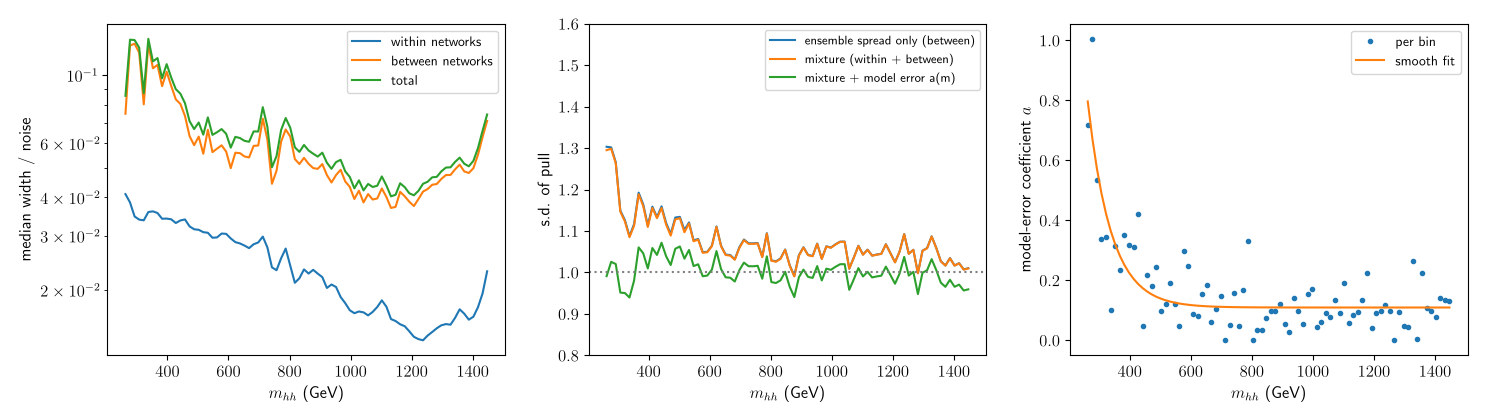
\includegraphics[width=\textwidth]{fig_laplace_summary.png}
\caption{Left: median width of the within-network, between-network and total predictive
uncertainty, in units of the noise. Middle: standard deviation of the pull on the 1,000 test
spectra for the ensemble spread alone, the mixture, and the mixture with the model-error term.
Right: the model-error coefficient per bin, determined on the quick-test rows, and its smooth
fit.}
\label{fig:summary}
\end{figure}

\paragraph{Calibration.} Without a model-error term the pulls have a standard deviation of 1.076
(1.15 near threshold), barely different from the ensemble alone (1.077): the parameter
uncertainty cannot account for the misfit. With
$a(m_{hh}) = 0.758\,e^{-(m_{hh} - 255)/76\,\text{GeV}} + 0.109$, fitted on the quick-test rows,
the standard deviation is 1.003 (1.023 and 0.996 below and above 555~GeV), and 95.1\% of the
bins have $|z| < 2$ (95.4\% for a normal distribution).

\begin{keyidea}[What this means for the paper]
The Bayesian treatment works and tells a clear story. Given this network and these data, the
parameters are well determined: about 400 effective parameters are fixed by
$2.8\times10^5$ rows, and each network's predictions are uncertain by only 2--3\% of the
POWHEG noise. Different equally good networks differ by about twice that. Both are small
compared with the error of the network form itself, 0.3--0.9 of the noise, which a posterior
over this network's parameters cannot describe and which must enter as a model-discrepancy
term. With it, the uncertainties are calibrated. The earlier Markov-chain widths are
explained: the chain under-explored its mode by a factor of five in width.
\end{keyidea}


% ===========================================================================
\section{The code}

\begin{itemize}
  \item \file{dihiggs/counts.py}: \code{recover\_counts}, \code{recover\_counts\_wide},
    \code{add\_empty\_bins}, \code{poisson\_variance}.
  \item \file{dihiggs/laplace.py}: \code{wilson\_coefficients}; the class \code{Laplace}
    with \code{fit\_hessian} (\code{method='factorised'} or \code{'rows'}),
    \code{set\_prior}, \code{fit\_prior}, \code{gamma}, \code{predict},
    \code{coeff\_covariance}, \code{log\_evidence}, \code{sample}, \code{evaluate},
    \code{eigenvalues}, \code{state}/\code{load\_state}; and \code{mixture}.
  \item \file{code/laplace_toy.py}: the exact-answer test.
  \item \file{code/heft_laplace.ipynb}: the whole calculation, the checks and the
    calibration. It runs on a laptop CPU in about 15 minutes for 20 networks and writes
    \file{runs/LAPLACE_<ensemble>/}.
\end{itemize}

\end{document}
